\documentclass{article} % For LaTeX2e
\usepackage{iclr2022_conference,times}
% Optional math commands from https://github.com/goodfeli/dlbook_notation.
%%%%% NEW MATH DEFINITIONS %%%%%

\usepackage{amsmath,amsfonts,bm}

% Mark sections of captions for referring to divisions of figures
\newcommand{\figleft}{{\em (Left)}}
\newcommand{\figcenter}{{\em (Center)}}
\newcommand{\figright}{{\em (Right)}}
\newcommand{\figtop}{{\em (Top)}}
\newcommand{\figbottom}{{\em (Bottom)}}
\newcommand{\captiona}{{\em (a)}}
\newcommand{\captionb}{{\em (b)}}
\newcommand{\captionc}{{\em (c)}}
\newcommand{\captiond}{{\em (d)}}

% Highlight a newly defined term
\newcommand{\newterm}[1]{{\bf #1}}


% Figure reference, lower-case.
\def\figref#1{figure~\ref{#1}}
% Figure reference, capital. For start of sentence
\def\Figref#1{Figure~\ref{#1}}
\def\twofigref#1#2{figures \ref{#1} and \ref{#2}}
\def\quadfigref#1#2#3#4{figures \ref{#1}, \ref{#2}, \ref{#3} and \ref{#4}}
% Section reference, lower-case.
\def\secref#1{section~\ref{#1}}
% Section reference, capital.
\def\Secref#1{Section~\ref{#1}}
% Reference to two sections.
\def\twosecrefs#1#2{sections \ref{#1} and \ref{#2}}
% Reference to three sections.
\def\secrefs#1#2#3{sections \ref{#1}, \ref{#2} and \ref{#3}}
% Reference to an equation, lower-case.
\def\eqref#1{equation~\ref{#1}}
% Reference to an equation, upper case
\def\Eqref#1{Equation~\ref{#1}}
% A raw reference to an equation---avoid using if possible
\def\plaineqref#1{\ref{#1}}
% Reference to a chapter, lower-case.
\def\chapref#1{chapter~\ref{#1}}
% Reference to an equation, upper case.
\def\Chapref#1{Chapter~\ref{#1}}
% Reference to a range of chapters
\def\rangechapref#1#2{chapters\ref{#1}--\ref{#2}}
% Reference to an algorithm, lower-case.
\def\algref#1{algorithm~\ref{#1}}
% Reference to an algorithm, upper case.
\def\Algref#1{Algorithm~\ref{#1}}
\def\twoalgref#1#2{algorithms \ref{#1} and \ref{#2}}
\def\Twoalgref#1#2{Algorithms \ref{#1} and \ref{#2}}
% Reference to a part, lower case
\def\partref#1{part~\ref{#1}}
% Reference to a part, upper case
\def\Partref#1{Part~\ref{#1}}
\def\twopartref#1#2{parts \ref{#1} and \ref{#2}}

\def\ceil#1{\lceil #1 \rceil}
\def\floor#1{\lfloor #1 \rfloor}
\def\1{\bm{1}}
\newcommand{\train}{\mathcal{D}}
\newcommand{\valid}{\mathcal{D_{\mathrm{valid}}}}
\newcommand{\test}{\mathcal{D_{\mathrm{test}}}}

\def\eps{{\epsilon}}


% Random variables
\def\reta{{\textnormal{$\eta$}}}
\def\ra{{\textnormal{a}}}
\def\rb{{\textnormal{b}}}
\def\rc{{\textnormal{c}}}
\def\rd{{\textnormal{d}}}
\def\re{{\textnormal{e}}}
\def\rf{{\textnormal{f}}}
\def\rg{{\textnormal{g}}}
\def\rh{{\textnormal{h}}}
\def\ri{{\textnormal{i}}}
\def\rj{{\textnormal{j}}}
\def\rk{{\textnormal{k}}}
\def\rl{{\textnormal{l}}}
% rm is already a command, just don't name any random variables m
\def\rn{{\textnormal{n}}}
\def\ro{{\textnormal{o}}}
\def\rp{{\textnormal{p}}}
\def\rq{{\textnormal{q}}}
\def\rr{{\textnormal{r}}}
\def\rs{{\textnormal{s}}}
\def\rt{{\textnormal{t}}}
\def\ru{{\textnormal{u}}}
\def\rv{{\textnormal{v}}}
\def\rw{{\textnormal{w}}}
\def\rx{{\textnormal{x}}}
\def\ry{{\textnormal{y}}}
\def\rz{{\textnormal{z}}}

% Random vectors
\def\rvepsilon{{\mathbf{\epsilon}}}
\def\rvtheta{{\mathbf{\theta}}}
\def\rva{{\mathbf{a}}}
\def\rvb{{\mathbf{b}}}
\def\rvc{{\mathbf{c}}}
\def\rvd{{\mathbf{d}}}
\def\rve{{\mathbf{e}}}
\def\rvf{{\mathbf{f}}}
\def\rvg{{\mathbf{g}}}
\def\rvh{{\mathbf{h}}}
\def\rvu{{\mathbf{i}}}
\def\rvj{{\mathbf{j}}}
\def\rvk{{\mathbf{k}}}
\def\rvl{{\mathbf{l}}}
\def\rvm{{\mathbf{m}}}
\def\rvn{{\mathbf{n}}}
\def\rvo{{\mathbf{o}}}
\def\rvp{{\mathbf{p}}}
\def\rvq{{\mathbf{q}}}
\def\rvr{{\mathbf{r}}}
\def\rvs{{\mathbf{s}}}
\def\rvt{{\mathbf{t}}}
\def\rvu{{\mathbf{u}}}
\def\rvv{{\mathbf{v}}}
\def\rvw{{\mathbf{w}}}
\def\rvx{{\mathbf{x}}}
\def\rvy{{\mathbf{y}}}
\def\rvz{{\mathbf{z}}}

% Elements of random vectors
\def\erva{{\textnormal{a}}}
\def\ervb{{\textnormal{b}}}
\def\ervc{{\textnormal{c}}}
\def\ervd{{\textnormal{d}}}
\def\erve{{\textnormal{e}}}
\def\ervf{{\textnormal{f}}}
\def\ervg{{\textnormal{g}}}
\def\ervh{{\textnormal{h}}}
\def\ervi{{\textnormal{i}}}
\def\ervj{{\textnormal{j}}}
\def\ervk{{\textnormal{k}}}
\def\ervl{{\textnormal{l}}}
\def\ervm{{\textnormal{m}}}
\def\ervn{{\textnormal{n}}}
\def\ervo{{\textnormal{o}}}
\def\ervp{{\textnormal{p}}}
\def\ervq{{\textnormal{q}}}
\def\ervr{{\textnormal{r}}}
\def\ervs{{\textnormal{s}}}
\def\ervt{{\textnormal{t}}}
\def\ervu{{\textnormal{u}}}
\def\ervv{{\textnormal{v}}}
\def\ervw{{\textnormal{w}}}
\def\ervx{{\textnormal{x}}}
\def\ervy{{\textnormal{y}}}
\def\ervz{{\textnormal{z}}}

% Random matrices
\def\rmA{{\mathbf{A}}}
\def\rmB{{\mathbf{B}}}
\def\rmC{{\mathbf{C}}}
\def\rmD{{\mathbf{D}}}
\def\rmE{{\mathbf{E}}}
\def\rmF{{\mathbf{F}}}
\def\rmG{{\mathbf{G}}}
\def\rmH{{\mathbf{H}}}
\def\rmI{{\mathbf{I}}}
\def\rmJ{{\mathbf{J}}}
\def\rmK{{\mathbf{K}}}
\def\rmL{{\mathbf{L}}}
\def\rmM{{\mathbf{M}}}
\def\rmN{{\mathbf{N}}}
\def\rmO{{\mathbf{O}}}
\def\rmP{{\mathbf{P}}}
\def\rmQ{{\mathbf{Q}}}
\def\rmR{{\mathbf{R}}}
\def\rmS{{\mathbf{S}}}
\def\rmT{{\mathbf{T}}}
\def\rmU{{\mathbf{U}}}
\def\rmV{{\mathbf{V}}}
\def\rmW{{\mathbf{W}}}
\def\rmX{{\mathbf{X}}}
\def\rmY{{\mathbf{Y}}}
\def\rmZ{{\mathbf{Z}}}

% Elements of random matrices
\def\ermA{{\textnormal{A}}}
\def\ermB{{\textnormal{B}}}
\def\ermC{{\textnormal{C}}}
\def\ermD{{\textnormal{D}}}
\def\ermE{{\textnormal{E}}}
\def\ermF{{\textnormal{F}}}
\def\ermG{{\textnormal{G}}}
\def\ermH{{\textnormal{H}}}
\def\ermI{{\textnormal{I}}}
\def\ermJ{{\textnormal{J}}}
\def\ermK{{\textnormal{K}}}
\def\ermL{{\textnormal{L}}}
\def\ermM{{\textnormal{M}}}
\def\ermN{{\textnormal{N}}}
\def\ermO{{\textnormal{O}}}
\def\ermP{{\textnormal{P}}}
\def\ermQ{{\textnormal{Q}}}
\def\ermR{{\textnormal{R}}}
\def\ermS{{\textnormal{S}}}
\def\ermT{{\textnormal{T}}}
\def\ermU{{\textnormal{U}}}
\def\ermV{{\textnormal{V}}}
\def\ermW{{\textnormal{W}}}
\def\ermX{{\textnormal{X}}}
\def\ermY{{\textnormal{Y}}}
\def\ermZ{{\textnormal{Z}}}

% Vectors
\def\vzero{{\bm{0}}}
\def\vone{{\bm{1}}}
\def\vmu{{\bm{\mu}}}
\def\vtheta{{\bm{\theta}}}
\def\va{{\bm{a}}}
\def\vb{{\bm{b}}}
\def\vc{{\bm{c}}}
\def\vd{{\bm{d}}}
\def\ve{{\bm{e}}}
\def\vf{{\bm{f}}}
\def\vg{{\bm{g}}}
\def\vh{{\bm{h}}}
\def\vi{{\bm{i}}}
\def\vj{{\bm{j}}}
\def\vk{{\bm{k}}}
\def\vl{{\bm{l}}}
\def\vm{{\bm{m}}}
\def\vn{{\bm{n}}}
\def\vo{{\bm{o}}}
\def\vp{{\bm{p}}}
\def\vq{{\bm{q}}}
\def\vr{{\bm{r}}}
\def\vs{{\bm{s}}}
\def\vt{{\bm{t}}}
\def\vu{{\bm{u}}}
\def\vv{{\bm{v}}}
\def\vw{{\bm{w}}}
\def\vx{{\bm{x}}}
\def\vy{{\bm{y}}}
\def\vz{{\bm{z}}}

% Elements of vectors
\def\evalpha{{\alpha}}
\def\evbeta{{\beta}}
\def\evepsilon{{\epsilon}}
\def\evlambda{{\lambda}}
\def\evomega{{\omega}}
\def\evmu{{\mu}}
\def\evpsi{{\psi}}
\def\evsigma{{\sigma}}
\def\evtheta{{\theta}}
\def\eva{{a}}
\def\evb{{b}}
\def\evc{{c}}
\def\evd{{d}}
\def\eve{{e}}
\def\evf{{f}}
\def\evg{{g}}
\def\evh{{h}}
\def\evi{{i}}
\def\evj{{j}}
\def\evk{{k}}
\def\evl{{l}}
\def\evm{{m}}
\def\evn{{n}}
\def\evo{{o}}
\def\evp{{p}}
\def\evq{{q}}
\def\evr{{r}}
\def\evs{{s}}
\def\evt{{t}}
\def\evu{{u}}
\def\evv{{v}}
\def\evw{{w}}
\def\evx{{x}}
\def\evy{{y}}
\def\evz{{z}}

% Matrix
\def\mA{{\bm{A}}}
\def\mB{{\bm{B}}}
\def\mC{{\bm{C}}}
\def\mD{{\bm{D}}}
\def\mE{{\bm{E}}}
\def\mF{{\bm{F}}}
\def\mG{{\bm{G}}}
\def\mH{{\bm{H}}}
\def\mI{{\bm{I}}}
\def\mJ{{\bm{J}}}
\def\mK{{\bm{K}}}
\def\mL{{\bm{L}}}
\def\mM{{\bm{M}}}
\def\mN{{\bm{N}}}
\def\mO{{\bm{O}}}
\def\mP{{\bm{P}}}
\def\mQ{{\bm{Q}}}
\def\mR{{\bm{R}}}
\def\mS{{\bm{S}}}
\def\mT{{\bm{T}}}
\def\mU{{\bm{U}}}
\def\mV{{\bm{V}}}
\def\mW{{\bm{W}}}
\def\mX{{\bm{X}}}
\def\mY{{\bm{Y}}}
\def\mZ{{\bm{Z}}}
\def\mBeta{{\bm{\beta}}}
\def\mPhi{{\bm{\Phi}}}
\def\mLambda{{\bm{\Lambda}}}
\def\mSigma{{\bm{\Sigma}}}

% Tensor
\DeclareMathAlphabet{\mathsfit}{\encodingdefault}{\sfdefault}{m}{sl}
\SetMathAlphabet{\mathsfit}{bold}{\encodingdefault}{\sfdefault}{bx}{n}
\newcommand{\tens}[1]{\bm{\mathsfit{#1}}}
\def\tA{{\tens{A}}}
\def\tB{{\tens{B}}}
\def\tC{{\tens{C}}}
\def\tD{{\tens{D}}}
\def\tE{{\tens{E}}}
\def\tF{{\tens{F}}}
\def\tG{{\tens{G}}}
\def\tH{{\tens{H}}}
\def\tI{{\tens{I}}}
\def\tJ{{\tens{J}}}
\def\tK{{\tens{K}}}
\def\tL{{\tens{L}}}
\def\tM{{\tens{M}}}
\def\tN{{\tens{N}}}
\def\tO{{\tens{O}}}
\def\tP{{\tens{P}}}
\def\tQ{{\tens{Q}}}
\def\tR{{\tens{R}}}
\def\tS{{\tens{S}}}
\def\tT{{\tens{T}}}
\def\tU{{\tens{U}}}
\def\tV{{\tens{V}}}
\def\tW{{\tens{W}}}
\def\tX{{\tens{X}}}
\def\tY{{\tens{Y}}}
\def\tZ{{\tens{Z}}}


% Graph
\def\gA{{\mathcal{A}}}
\def\gB{{\mathcal{B}}}
\def\gC{{\mathcal{C}}}
\def\gD{{\mathcal{D}}}
\def\gE{{\mathcal{E}}}
\def\gF{{\mathcal{F}}}
\def\gG{{\mathcal{G}}}
\def\gH{{\mathcal{H}}}
\def\gI{{\mathcal{I}}}
\def\gJ{{\mathcal{J}}}
\def\gK{{\mathcal{K}}}
\def\gL{{\mathcal{L}}}
\def\gM{{\mathcal{M}}}
\def\gN{{\mathcal{N}}}
\def\gO{{\mathcal{O}}}
\def\gP{{\mathcal{P}}}
\def\gQ{{\mathcal{Q}}}
\def\gR{{\mathcal{R}}}
\def\gS{{\mathcal{S}}}
\def\gT{{\mathcal{T}}}
\def\gU{{\mathcal{U}}}
\def\gV{{\mathcal{V}}}
\def\gW{{\mathcal{W}}}
\def\gX{{\mathcal{X}}}
\def\gY{{\mathcal{Y}}}
\def\gZ{{\mathcal{Z}}}

% Sets
\def\sA{{\mathbb{A}}}
\def\sB{{\mathbb{B}}}
\def\sC{{\mathbb{C}}}
\def\sD{{\mathbb{D}}}
% Don't use a set called E, because this would be the same as our symbol
% for expectation.
\def\sF{{\mathbb{F}}}
\def\sG{{\mathbb{G}}}
\def\sH{{\mathbb{H}}}
\def\sI{{\mathbb{I}}}
\def\sJ{{\mathbb{J}}}
\def\sK{{\mathbb{K}}}
\def\sL{{\mathbb{L}}}
\def\sM{{\mathbb{M}}}
\def\sN{{\mathbb{N}}}
\def\sO{{\mathbb{O}}}
\def\sP{{\mathbb{P}}}
\def\sQ{{\mathbb{Q}}}
\def\sR{{\mathbb{R}}}
\def\sS{{\mathbb{S}}}
\def\sT{{\mathbb{T}}}
\def\sU{{\mathbb{U}}}
\def\sV{{\mathbb{V}}}
\def\sW{{\mathbb{W}}}
\def\sX{{\mathbb{X}}}
\def\sY{{\mathbb{Y}}}
\def\sZ{{\mathbb{Z}}}

% Entries of a matrix
\def\emLambda{{\Lambda}}
\def\emA{{A}}
\def\emB{{B}}
\def\emC{{C}}
\def\emD{{D}}
\def\emE{{E}}
\def\emF{{F}}
\def\emG{{G}}
\def\emH{{H}}
\def\emI{{I}}
\def\emJ{{J}}
\def\emK{{K}}
\def\emL{{L}}
\def\emM{{M}}
\def\emN{{N}}
\def\emO{{O}}
\def\emP{{P}}
\def\emQ{{Q}}
\def\emR{{R}}
\def\emS{{S}}
\def\emT{{T}}
\def\emU{{U}}
\def\emV{{V}}
\def\emW{{W}}
\def\emX{{X}}
\def\emY{{Y}}
\def\emZ{{Z}}
\def\emSigma{{\Sigma}}

% entries of a tensor
% Same font as tensor, without \bm wrapper
\newcommand{\etens}[1]{\mathsfit{#1}}
\def\etLambda{{\etens{\Lambda}}}
\def\etA{{\etens{A}}}
\def\etB{{\etens{B}}}
\def\etC{{\etens{C}}}
\def\etD{{\etens{D}}}
\def\etE{{\etens{E}}}
\def\etF{{\etens{F}}}
\def\etG{{\etens{G}}}
\def\etH{{\etens{H}}}
\def\etI{{\etens{I}}}
\def\etJ{{\etens{J}}}
\def\etK{{\etens{K}}}
\def\etL{{\etens{L}}}
\def\etM{{\etens{M}}}
\def\etN{{\etens{N}}}
\def\etO{{\etens{O}}}
\def\etP{{\etens{P}}}
\def\etQ{{\etens{Q}}}
\def\etR{{\etens{R}}}
\def\etS{{\etens{S}}}
\def\etT{{\etens{T}}}
\def\etU{{\etens{U}}}
\def\etV{{\etens{V}}}
\def\etW{{\etens{W}}}
\def\etX{{\etens{X}}}
\def\etY{{\etens{Y}}}
\def\etZ{{\etens{Z}}}

% The true underlying data generating distribution
\newcommand{\pdata}{p_{\rm{data}}}
% The empirical distribution defined by the training set
\newcommand{\ptrain}{\hat{p}_{\rm{data}}}
\newcommand{\Ptrain}{\hat{P}_{\rm{data}}}
% The model distribution
\newcommand{\pmodel}{p_{\rm{model}}}
\newcommand{\Pmodel}{P_{\rm{model}}}
\newcommand{\ptildemodel}{\tilde{p}_{\rm{model}}}
% Stochastic autoencoder distributions
\newcommand{\pencode}{p_{\rm{encoder}}}
\newcommand{\pdecode}{p_{\rm{decoder}}}
\newcommand{\precons}{p_{\rm{reconstruct}}}

\newcommand{\laplace}{\mathrm{Laplace}} % Laplace distribution

\newcommand{\E}{\mathbb{E}}
\newcommand{\Ls}{\mathcal{L}}
\newcommand{\R}{\mathbb{R}}
\newcommand{\emp}{\tilde{p}}
\newcommand{\lr}{\alpha}
\newcommand{\reg}{\lambda}
\newcommand{\rect}{\mathrm{rectifier}}
\newcommand{\softmax}{\mathrm{softmax}}
\newcommand{\sigmoid}{\sigma}
\newcommand{\softplus}{\zeta}
\newcommand{\KL}{D_{\mathrm{KL}}}
\newcommand{\Var}{\mathrm{Var}}
\newcommand{\standarderror}{\mathrm{SE}}
\newcommand{\Cov}{\mathrm{Cov}}
% Wolfram Mathworld says $L^2$ is for function spaces and $\ell^2$ is for vectors
% But then they seem to use $L^2$ for vectors throughout the site, and so does
% wikipedia.
\newcommand{\normlzero}{L^0}
\newcommand{\normlone}{L^1}
\newcommand{\normltwo}{L^2}
\newcommand{\normlp}{L^p}
\newcommand{\normmax}{L^\infty}

\newcommand{\parents}{Pa} % See usage in notation.tex. Chosen to match Daphne's book.

\DeclareMathOperator*{\argmax}{arg\,max}
\DeclareMathOperator*{\argmin}{arg\,min}

\DeclareMathOperator{\sign}{sign}
\DeclareMathOperator{\Tr}{Tr}
\let\ab\allowbreak


%######## APS360: Uncomment your submission name
\newcommand{\apsname}{Final Report}
%\newcommand{\apsname}{Progress Report}
%\newcommand{\apsname}{Final Report}

%######## APS360: Put your Group Number here
\newcommand{\gpnumber}{4}
\usepackage{float}
\usepackage{hyperref}
\usepackage{url}
\usepackage{graphicx}

%######## APS360: Put your project Title here
\title{Autonomous Car Using Deep Learning - \\Final Report}


%######## APS360: Put your names, student IDs and Emails here
\author{Rudra Dey  \\
Student\# 1010124866\\
\texttt{rudra.dey@mail.utoronto.ca } \\
\And
Pravin Kalaivannan  \\
Student\# 1010141295 \\
\texttt{pravin.kalaivannan@mail.utoronto.ca} \\
\AND
Aadavan Vasudevan  \\
Student\# 1010101514 \\
\texttt{aadavan.vasudevan@mail.utoronto.ca} \\
\And
Abishan Baheerathan \\
Student\# 1010218756 \\
\texttt{abishan.baheerathan@mail.utoronto.ca} \\
\AND
}

% The \author macro works with any number of authors. There are two commands
% used to separate the names and addresses of multiple authors: \And and \AND.
%
% Using \And between authors leaves it to \LaTeX{} to determine where to break
% the lines. Using \AND forces a linebreak at that point. So, if \LaTeX{}
% puts 3 of 4 authors names on the first line, and the last on the second
% line, try using \AND instead of \And before the third author name.

\newcommand{\fix}{\marginpar{FIX}}
\newcommand{\new}{\marginpar{NEW}}

\iclrfinalcopy 
%######## APS360: Document starts here
\begin{document}


\maketitle

%######## APS360: Do not change the next line. This shows your Main body page count.
Total Pages: \pageref{last_page}


\section{Introduction}

In 2023, the Toronto Police Service reported 298 vehicle collisions which led to death (or serious injury) within that year \citep{toronto-ksi}. This data seems illogical when
you find out that Toronto’s rated safety score is 4.4 out of 5 compared to other cities in Ontario \citep{brokerlink2025ontario}.
This depressing reality of what a safe city is considered was our motivation to make this project about the creation of autonomous self-driving cars. To have self-driving cars be deployed and widely adopted in any urban city would significantly reduce traffic accidents.

In the short term, it is impossible to replace all human-driven cars with self-driven cars, instead a city needs to adopt the idea and slowly
create infrastructure which supports these self-driving cars. Machine learning is a well-suited approach for this task because having a mix of
self-driven cars and human-driven cars ultimately still involves human error, and thus requires on the spot judgement. A traditional rule based
system will struggle to handle the wide variety of edge cases that occur on the road. Deep learning on the other hand enables the car to learn
complex patterns from data and make rapid decisions. By using CNNs we can create a system which interprets multimodal inputs such as RGB camera
sensors and indicator signal state, and then predict appropriate driving behaviour.

\section{Illustration}


\begin{figure}[H] % h = here, t = top, b = bottom, p = page of floats
    \centering
    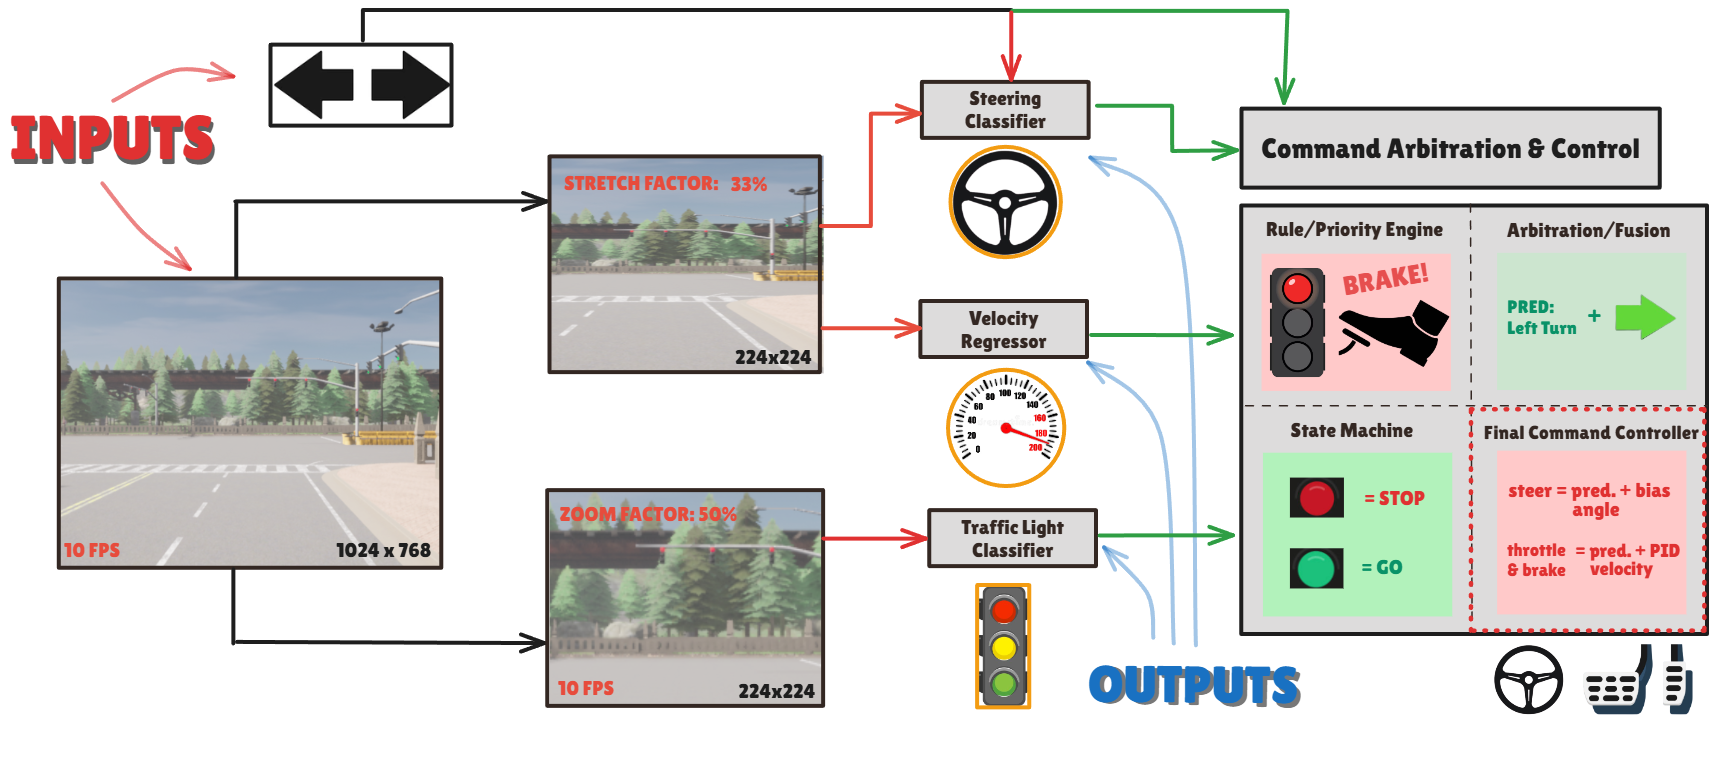
\includegraphics[width=1.0\textwidth]{newPic.png} % Adjust path and size
    \caption{Overall illustration of the autonomous driving system.}
    \label{fig:illustrationExample}
\end{figure}

\section{Background \& Related Work}
Our autonomous self-driving car is a multimodal system, which predicts three outputs: steering angle, speed, and traffic light colour.
This formulation puts our work in between two research fields in autonomous driving: raw-sensory input driving and control-oriented signalled driving.
The following is an overview of five works related to these fields.

\subsection{Vision-Based Multi-task Perception \citep{3.1Ref}}
Recent studies have shown that multi-task learning can improve efficiency in autonomous driving by allowing a shared backbone to
handle several perception and control tasks simultaneously. For example, models such as MultiNet and YOLOP perform object detection and
lane segmentation, showing that the feature sharing reduces redundancy while maintaining real-time performance. Inspired by this approach,
our project adopts a multi-head architecture that predicts steering, speed, and traffic-light state from a single camera input.

\subsection{NVIDIA PilotNet Experiments \citep{3.2Ref}}
NVIDIA’s PilotNet by Bojarski et al. demonstrated that a CNN could map front-facing camera images
directly to steering commands for lane detection and following.
This showed that deep networks could replace hand-engineered pipelines for this task.

\subsection{Conditional Imitation Learning \citep{3.3Ref}}
Codevilla introduced Conditional Imitation Learning (CIL), which extended autonomous driving by conditioning the policy
on higher-level navigation commands. The work showed that multi-task learning and structured outputs could be generalized
in simulated urban driving. In our approach, we trained primarily via imitation learning, producing three outputs that were
fed into a higher-level navigation module. This module applies conditional statements, which then control the car.

\subsection{Traffic Light Detection \citep{3.4Ref}}
The team uses deep CNNs to classify signal states from camera crops. The problem of detecting and classifying traffic lights is a
well-studied problem, and hard-engineered pipelines require specialized detectors and regional proposals. This showed that using a
CNN a lightweight traffic-light classifier can be created, and that is what we did with high accuracy.

\subsection{DeepDriving: Learning Affordance in Autonomous Driving \citep{3.5Ref}}
DeepDriving is an approach for autonomous driving which predicts intermediate affordances, such as the distance to
lane markings or the state of traffic lights, rather than controlling the car directly. We extended this idea and used
models to predict steering angles, traffic-light states, and speed, which is then passed through a higher-level navigation
command module, which then controls the car after conditions are met.


\section{Data Processing}

Data was collected from the CARLA simulator through the use of cameras and sensors, which makes up three different dataset types. We then normalized and resized the image as part of the preprocessing setup to implement the data into our network. Data augmentation techniques were then applied to force the traffic light model to learn deeper patterns.

\subsection{Data Collection and Cleaning}
This project required the team to gather five total datasets through the CARLA simulator: steering, velocity, traffic light, manual driving
and finally a test dataset which included data from all four types of datasets. Four Python scripts were written to enable the process by 
which the data was collected. We attached RGB camera sensors to the car to record at 10 frames per second (FPS) as the car travels around 
designated maps, either through the built-in autopilot functionality or manual driving (for the manual driving dataset). In addition to the camera, 
sensors on the car collect necessary data for said dataset, such as velocity at that frame. The data collected from the sensors was used for ground 
truth labels, allowing the model to be trained. A single dataset is made up of various maps, which is done by saving an individual map’s data as numpy 
files, then concatenating all the maps sequentially, creating one large dataset. Along with this data, our model needs live data collection for the steering signals.
These turn signals are collected through a keyboard input, and sent to the model to bias the turning angle.

To ensure the data was not corrupted, scripts were created to visualize the images along with the associated ground truth labels. A numpy file viewer was also used to ensure the ground truth labels varied, meaning that the dataset was diverse.

\begin{table}[h]
\centering
\caption{Datasets and their associated data types}
\vspace{0.5em}
\begin{tabular}{|p{5cm}|p{7cm}|}
\hline
\textbf{Type of Dataset} & \textbf{Data Collected in a Frame} \\ \hline
Steering Dataset & Images, Angles, Turn Signals \\ \hline
Velocity Dataset & Images, Velocities \\ \hline
Intersection Light Dataset & Images, State Labels \\ \hline
Manual Driving Dataset & Images, Angles, Turn Signals, Velocities \\ \hline
\end{tabular}
\end{table}


\subsection{Data Preprocessing}

All collected images were resized to a resolution of 224x224x3 as shown in \autoref{fig:datasetExample}, with pixel values normalized to a range of [0, 1].
This was done to ensure that the images can be used with the ResNet18 backbone, allowing for use in our deep learning model. In addition to this, for the traffic light dataset, all images had the left and right sides blurred, along with a \(\frac{1}{3}\) cropping of the bottom of the image, as shown in \autoref{fig:datasetExample}. This was done to ensure the traffic light model learns the behaviour and patterns of the light ahead of it, while disregarding other signals' views.

\begin{figure}[H] % h = here, t = top, b = bottom, p = page of floats
    \centering
    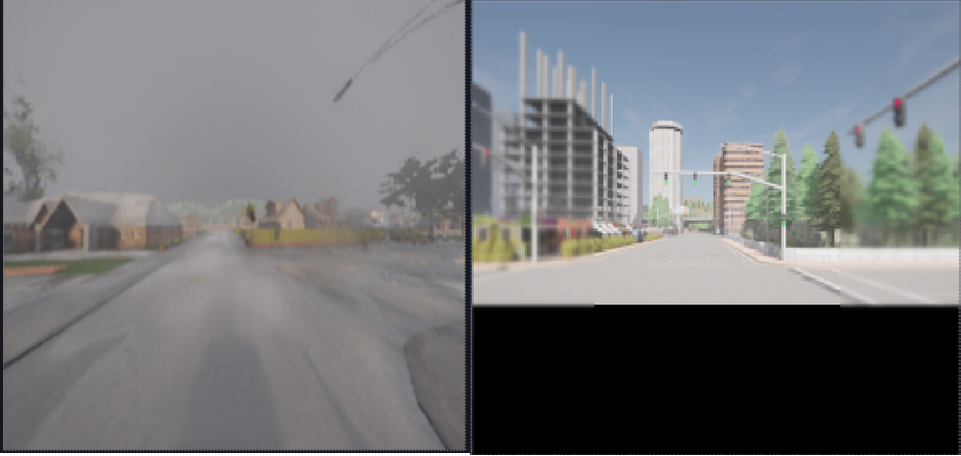
\includegraphics[width=1.0\textwidth]{example of images in dataset.png} % Adjust path and size
    \caption{Preprocessed images: Steering/Velocity image (left), Intersection Light image (right).}
    \label{fig:datasetExample}
\end{figure}


\subsection{Data Distribution}

The datasets were split 80/20 for the training and validation sets, respectively, which ensured we have a large set of data to train the model, while having enough data for validating its performance. In addition, a separate test dataset was collected, containing a number of samples of the various types of data. 
This data was collected on an unused map (not seen in training or validation), allowing the team to test the performance of the model on unseen data. The test dataset also includes data from the manual dataset, which was split into its respective data types (steering, and velocity).
All datasets were uploaded to a shared OneDrive so all members can access them as needed. Below, \autoref{tab:dataset_distribution} shows the distribution of the data. 

\begin{table}[H]
    \centering
    \caption{Dataset Distribution}
    \label{tab:dataset_distribution}
    \vspace{0.5em}
    \begin{tabular}{|l|p{2.5cm}|p{2.5cm}|r|r|}
        \hline
        \textbf{Dataset Type}      & \centering\textbf{Training   Samples} \newline \textbf{(80\%)} & \centering\textbf{Validation    Samples} \newline \textbf{(20\%)} & \textbf{Test Samples} & \textbf{Total Samples} \\ \hline
        Steering Dataset           & \centering 17,898                                              & \centering 4,474                                                  & 6,386                 & 28,758                 \\ \hline
        Velocity Dataset           & \centering 56,000                                              & \centering 14,000                                                 & 8,000                 & 78,000                 \\ \hline
        Intersection Light Dataset & \centering 1,966                                               & \centering 491                                                    & 492                   & 2,949                  \\ \hline
        \textbf{Total}             & \centering\textbf{75,864}                                      & \centering\textbf{18,965}                                         & \textbf{14,878}       & \textbf{109,707}       \\ \hline
    \end{tabular}
\end{table}

\subsection{Data Augmentation}

The team iterated through different data augmentation techniques when training the models, and in the end decided to only augment the intersection light dataset for training.

For the steering and velocity models, the environmental context and surrounding structures are critical for how the model learns driving behaviours. If augmentations were applied to the images in the associated datasets, it would cause the model to pick up on the wrong patterns and learn bad driving behaviours, such as driving on the opposite side of the road if the augmentation was a horizontal flip.

In contrast, the intersection light dataset benefits from augmentations.  A mix of augmentations was applied to ensure that the model learns the correct signal patterns. These augmentation techniques include brightness and contrast adjustment, horizontal flips, random rotation and cutouts. These augmentations, shown in \autoref{fig:dataaugmentation}, allowed the model to learn deeper traffic light features,  significantly improving its effectiveness.

\begin{figure}[H] % h = here, t = top, b = bottom, p = page of floats
    \centering
    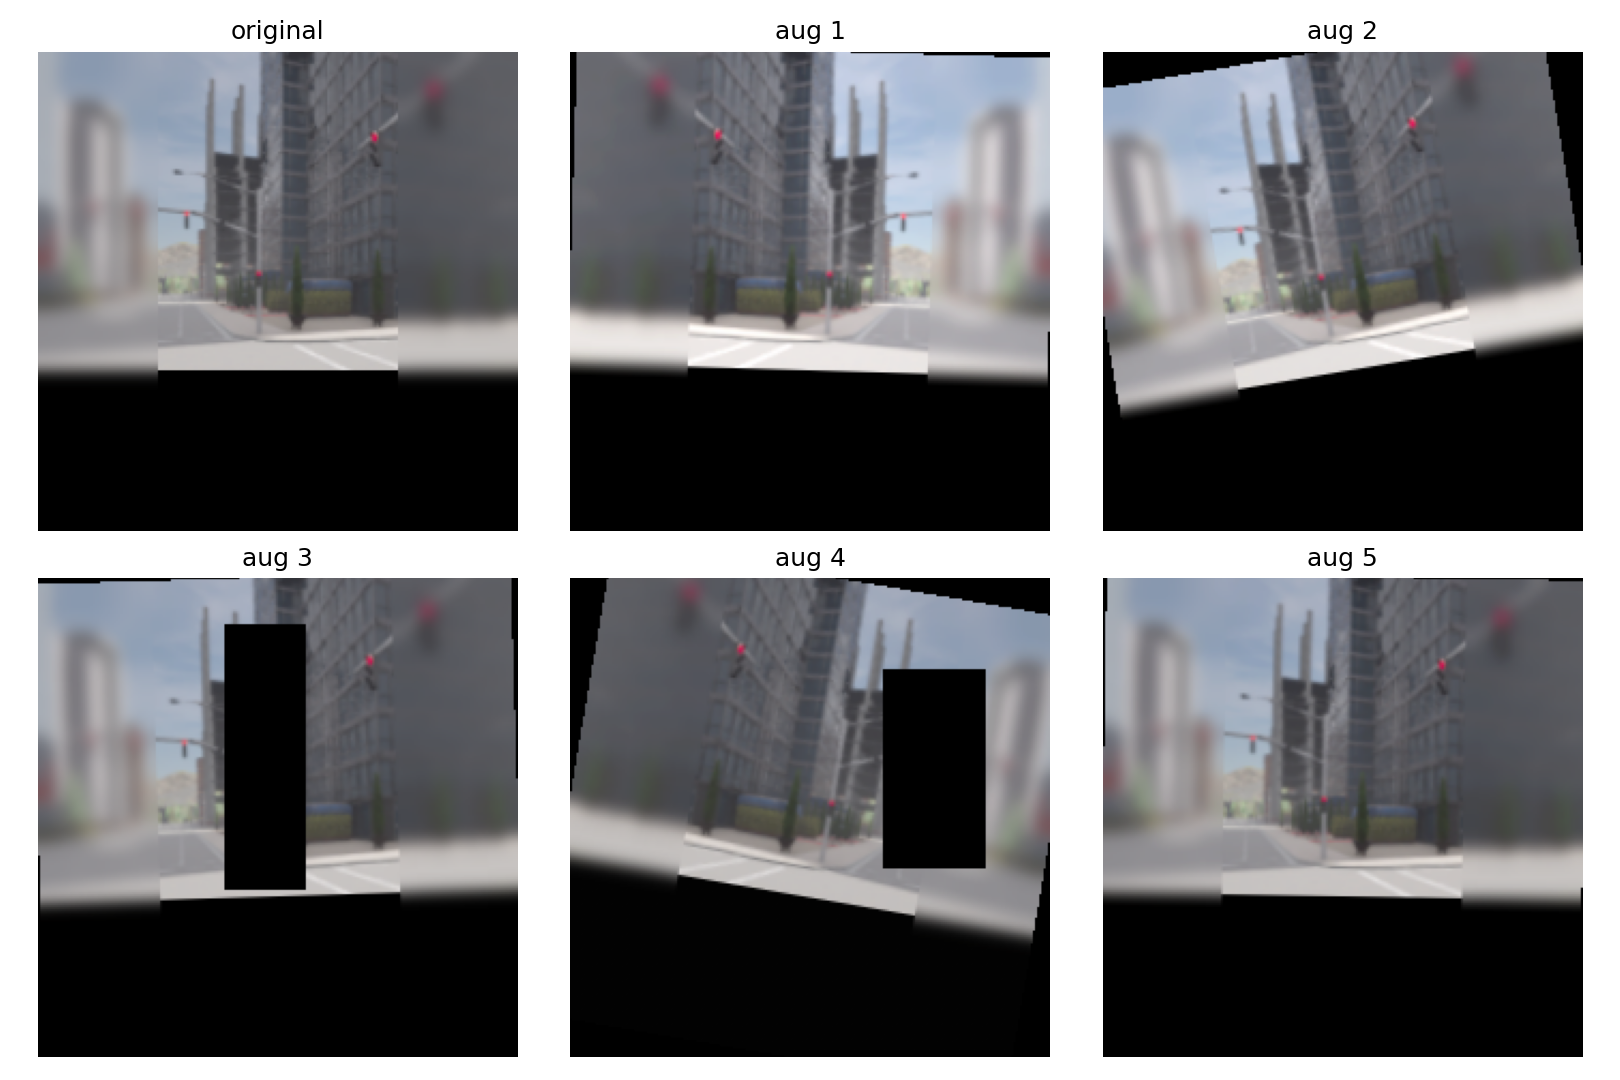
\includegraphics[width=1.0\textwidth]{Data Augmentation.png} % Adjust path and size
    \caption{Example of Data Augmentation Techniques on Intersection Light Dataset}
    \label{fig:dataaugmentation}
\end{figure}

\section{Architecture}

As shown in \autoref{fig:GoogleDrawingPrimaryArchyDiagram} , our project uses three separate deep learning models, velocity prediction, traffic light classification, and steering angle prediction.
All models are built on a shared convolutional backbone of ResNet-18 which is pretrained on ImageNet. ResNet was selected for its strong low-level and mid-level feature extraction ability, particularly in structured domains such as road images.

\begin{figure}[H] % h = here, t = top, b = bottom, p = page of floats
    \centering
    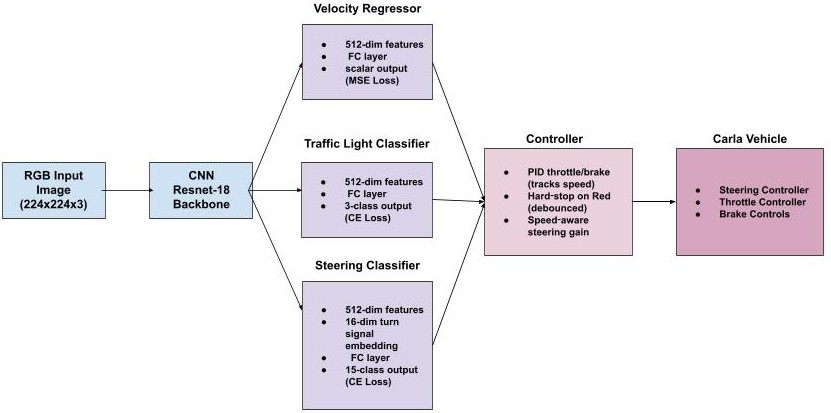
\includegraphics[width=1.0\textwidth]{GoogleDrawingPrimaryArchyDiagram.jpg} % Adjust path and size
    \caption{Final Architecture Low Level Diagram}
    \label{fig:GoogleDrawingPrimaryArchyDiagram}
\end{figure}

\subsection{Transfer Learning with ResNet-18}

The ResNet-18 backbone processes each 224x224 dimensioned RGB frame to produce a 512- dimensional feature vector.
For our application, only the convolutional layers of ResNet-18 are retained. In the early stages of training, these layers are frozen to preserve pretrained weights, with selective unfreezing applied during fine-tuning to adapt to the driving domain.

\subsection{Velocity Regressor}
The velocity regressor receives the 512-dimensional feature vector and processes it through a two-layer fully connected network with a ReLU activation between layers.
The first layer reduces dimensionality from 512 to 256 units, and the second produces a single scalar velocity value. Mean Squared Error (MSE)
loss is applied during training to encourage accurate continuous speed prediction.

\subsection{Steering Classifier}
For steering control, the 512-dimensional backbone output is concatenated with a 16-dimensional learned turn-signal embedding, producing a 528-dimensional input vector.
This vector passes through a fully connected layer reducing it to 256 units, followed by a ReLU activation, and finally a fully connected layer outputting logits for 15 discrete steering angle bins.
Cross-Entropy loss is used for classification

\subsection{Traffic Light Classifier}

The traffic light classifier head reduces the 512-dimensional input to 256 via a fully connected layer with ReLU activation, followed by a final fully connected layer outputting probabilities for three traffic light states (Red, Green and No-Light).
Cross-Entropy loss drives this classification task.

\subsection{Parameter Breakdown}

\autoref{fig:LayerTable} summarizes the custom fully connected layers in each prediction head, excluding the ResNet-18 backbone parameters (~11M).

\begin{table}[H] % h = here, t = top, b = bottom, p = page of floats
    \centering
    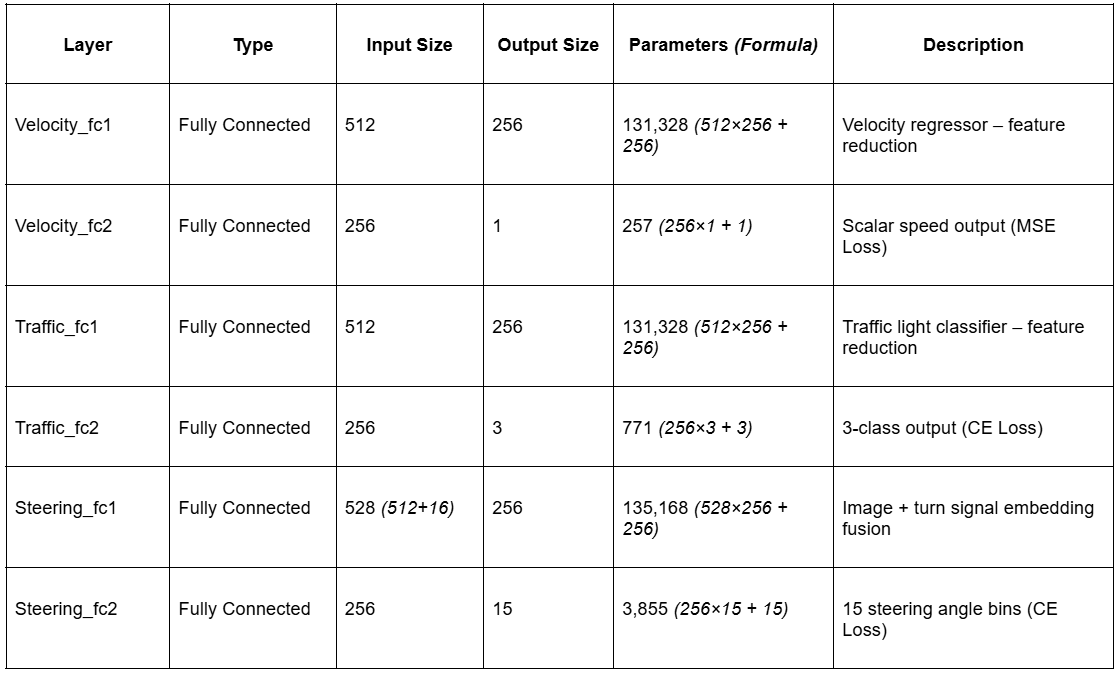
\includegraphics[width=1.0\textwidth]{LayerTable.png} % Adjust path and size
    \caption{Final Architecture Low Level Diagram}
    \label{fig:LayerTable}
\end{table}

\subsection{Quantitative Results}

\subsection{Qualitative Results}

\section{Baseline Model}

Using a Ridge Regression Algorithm we created a baseline model that predicts steering angles for a self-driving car
from grayscale camera images and turn signal inputs. This baseline model serves as a simple, interpretable baseline
such that we can compare our more complex primary neural network model later. To collect data, we used a simulator
called CARLA, to obtain camera images, turn signal inputs, and our ground truth label for the steering angles.


\subsection{Ridge Regression with Image Features}

In the model outlined in \autoref{fig:diagram}, the grayscale images (of shape 160x120) were flattened into 1D feature vectors and normalized. The features themselves
represent the visual input of the car's front-facing camera. Additionally, left and right turning signals were captured as an
additional feature; combining this with our flattened grayscale images we were left with a numpy array of shape $N \times 19201$,
where $N$ represents the number of images, and 19201 are the number of feature column vectors. The Ridge Regression algorithm was
selected because it penalized large coefficients ($L_2$ norm), allowing for a generalized model. A series of models were trained
with different regularization strengths ($\alpha$), and the performance was evaluated using Mean Squared Error (MSE) and $R^2$ Score
on a held-out 20\% test set.

\begin{figure}[H] % h = here, t = top, b = bottom, p = page of floats
    \centering
    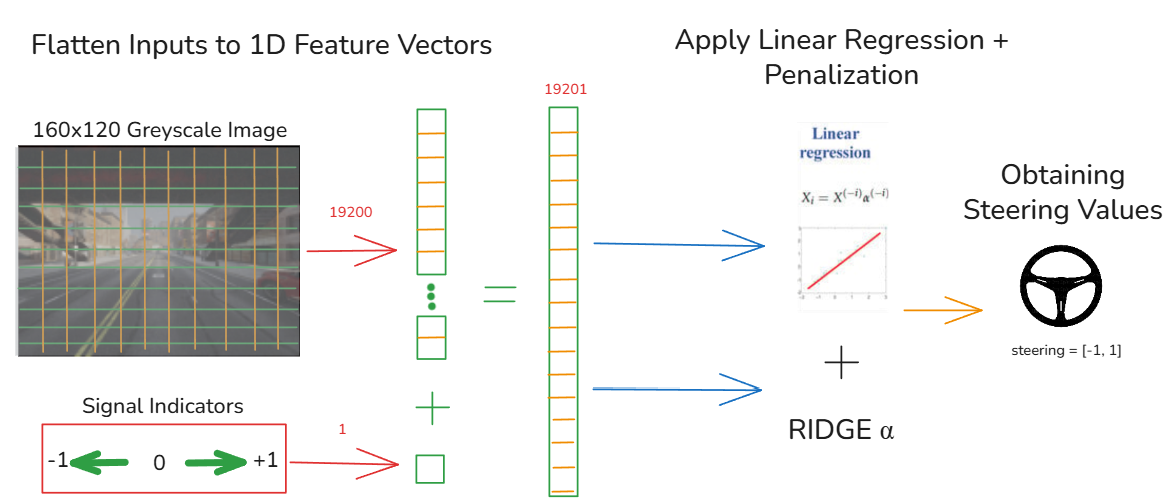
\includegraphics[width=1.0\textwidth]{diagram.png} % Adjust path and size
    \caption{Basic Architecture of Steering Angle  Ridge Regrsession Model}
    \label{fig:diagram}
\end{figure}


\subsection{Minimal Tuning of $\alpha$}
The only hyperparameter needing to be tuned was the regularization strength for the Ridge Regression Algorithm. This was manually tuned,
and thus no validation set was used. A small set of candidate values for $\alpha$ was chosen: $\alpha \text{ } \epsilon \text{ }
    \{ 1, 10, 100, 250, 1000, 8000\}$ With each value of $\alpha$, the model was trained and tested with a dataset of 15 minutes of simulated
driving. By obtaining the average MSE and the average $R^2$ score, our fourth model of $\alpha = 100$ came out to be the best.


\begin{figure}[H] % h = here, t = top, b = bottom, p = page of floats
    \centering
    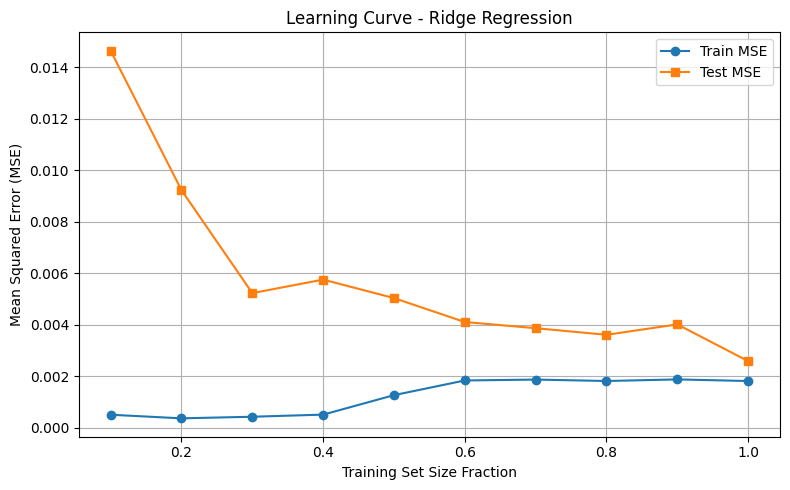
\includegraphics[width=0.6\textwidth]{model4learningcurve.png} % Adjust path and size
    \caption{This is the learning curve for "Model 4" a Ridge Regression Model with $\alpha = 100$}
    \label{fig:model4learningcurve}
\end{figure}

\subsection{Overfitting and Model Quality}
As shown in \autoref{fig:model4learningcurve}, the results suggest some overfitting due to the model's tendency
to perform much better on training data than unseen data. This is reasonable since the training data frames,
are all consecutive in nature, and the dataset used isn't extremely large either. In addition, as the training size
increases the gap between Test and Train MSEs narrows, suggesting that with more data the model will generalize better.
The final test MSE is (~0.0025) which is quite low, meaning the model performs well overall after training on the data.


\subsection{Qualitative Observations}
When running the steering angle prediction model in the CARLA simulator, the model exhibited promising behaviour in terms of
autonomous driving capabilities, however with large limitations. The car was able to drive freely, using the model's predictions
from the front-facing grayscale camera images and turn signals provided by the user. In \autoref{fig:model4demo} we can see
the model taking a left turn in an intersection.

\begin{itemize}
    \item \textbf{Turn Signal Response:} The car consistently turned in the correct direction when prompted, showing that the model incorporated turn signal input effectively.

    \item \textbf{Obstacle Avoidance:} The vehicle generally avoided obstacles but occasionally clipped walls, suggesting basic spatial awareness but limited precision.

    \item \textbf{Lane-Keeping:} The car had trouble staying within lane boundaries, often drifting, especially during turns or on complex roads.

    \item \textbf{Map Generalization:} Despite limitations, the car performed reasonably well across different map layouts, showing decent control over turns.
\end{itemize}


\begin{figure}[H] % h = here, t = top, b = bottom, p = page of floats
    \centering
    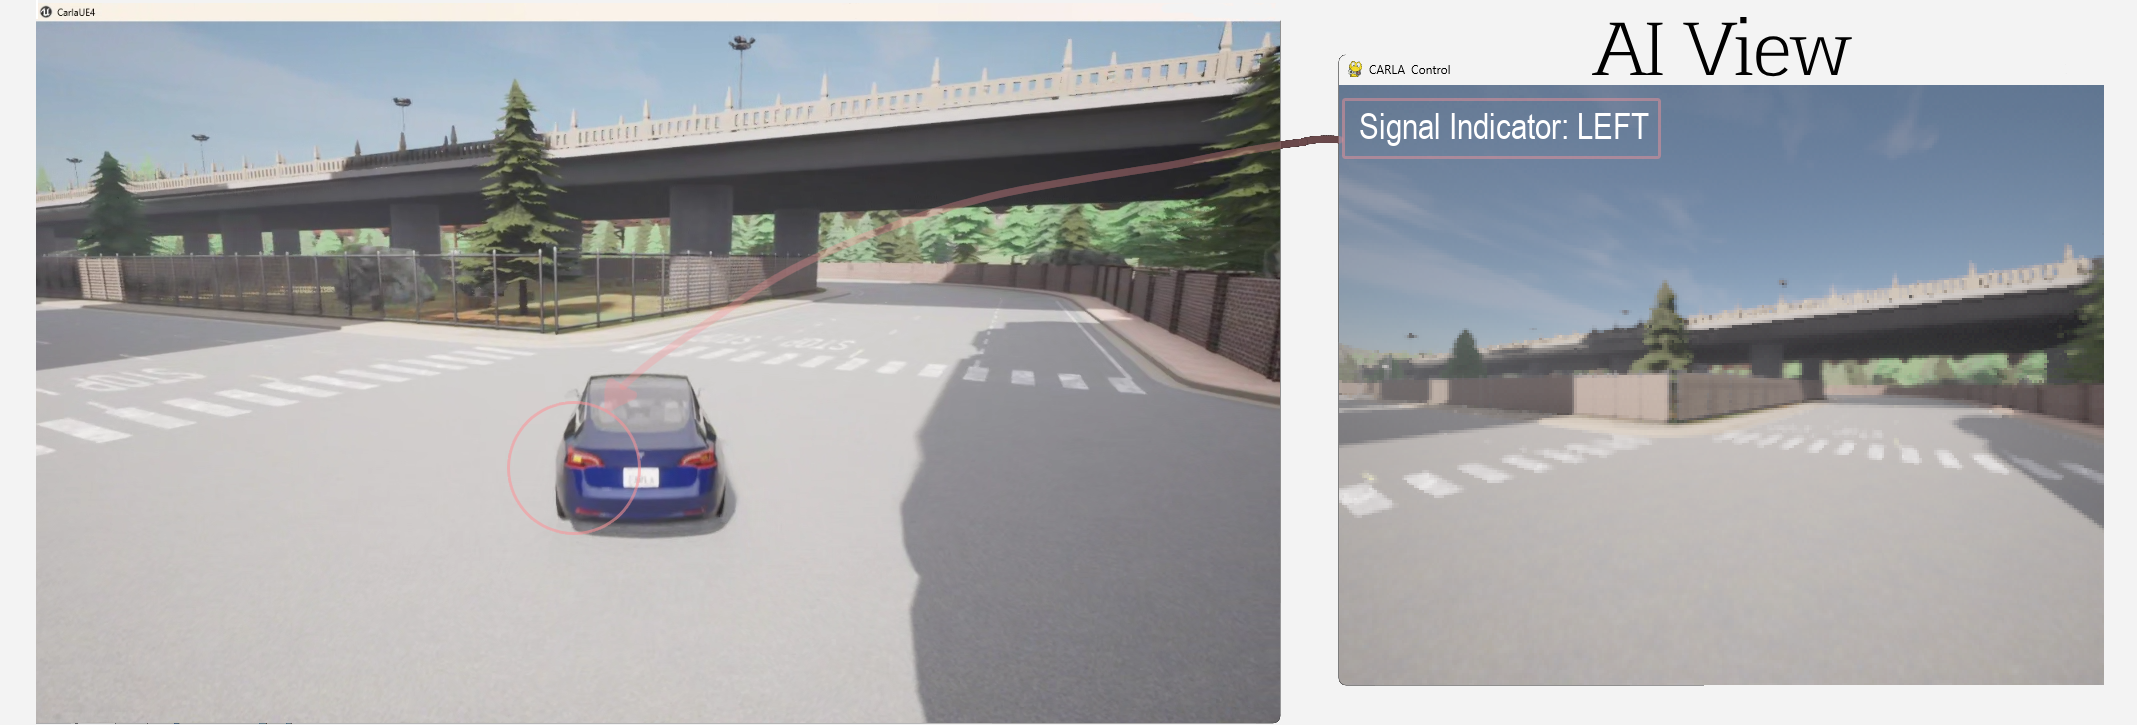
\includegraphics[width=1.0\textwidth]{model4demo.png} % Adjust path and size
    \caption{This is the demo for "Model 4" in CARLA}
    \label{fig:model4demo}
\end{figure}


\section{Evaluation on Test Data}
A test dataset was collected, made up of all the different dataset types (steering, velocity and traffic lights). 
This dataset contains data from an unused map, ensuring that it is unseen data.
The images were then normalized and resized to 224x244x3in the same preprocessing as the training and validation data.

\subsection{Test Results}
Individual tests were run on the models to determine their performance, and the results are shown below:

\begin{itemize}
    \item \textbf{Steering Classifier:}
    \begin{itemize}
        \item Test Accuracy: 53.10\%
        \item Cross Entropy (CE) Loss: 1.792
    \end{itemize}

    \item \textbf{Intersection Light Classifier}
    \begin{itemize}
        \item Test Accuracy: 99.80\%
        \item CE Loss: 0.0457
    \end{itemize}

    \item \textbf{Velocity Regressor:}
    \begin{itemize}
        \item Mean Absolute Error (MAE) = 0.9614
        \item Mean Square Error (MSE) = 1.7538
        \item R\textsuperscript{2} = 85.24\%
    \end{itemize}
\end{itemize}

\subsection{Results Evaluation}
For the Steering Classifier, the test resulted in an accuracy of 53.10\%, 
which is lower than our expectations, but is reasonable given the complexity of the problem. As we output 15 classes, 
slight deviations in steering values can cause the predictions to fall into adjacent bins, lowering accuracy. 
Additionally, the model is designed to take in human input for steering values through turn signals. 
These signals bias the turning, making the model turn more, and as we are unable to apply these signals during testing, 
it might lead to a lower test accuracy. With a CE of 1.792 across the 15 classes, it is clear that the model learned some meaningful patterns, 
though it is not perfect.

The Intersection Light Classifier ended up with excellent results with a near-perfect test accuracy along with a CE loss of 0.0457. 
This shows that the classifier has learned deep features and is reliable at detecting the state of traffic lights. 

The results of the Velocity Regressor meet expectations, with an MAE of 0.9614, meaning that the predictions were on average 0.96 m/s 
off the actual value, which is within our expectations. With a low MSE of 1.7538, it shows that the errors are not large discrepancies. 
Additionally, the $R^2$ of 85.24\% shows the model captures the majority of the variation in velocity, demonstrating strong performance. 


\section{Discussion of Results}

The results that the team collected show that our models performed well given the specific tasks that
they had to complete. The steering classifier achieved an accuracy of 53.10\%, the intersection light
classifier achieved 99.80\%, and the velocity regressor had a R\textsuperscript{2} of 0.8524. The steering
classifier accuracy is still impressive because of how difficult it is to predict steering angles and
the different driving conditions. These results show that our system works well together and has
achieved great results.

We implemented multimodal data by combining visual and sensor data. This was interesting because of how
the models improved significantly. The system was able to capture crucial information in certain driving
situations because of the multimodal data. This improved the system’s accuracy because it helped provide
more context for the models.

An important lesson that the team learned was to balance regression and classification loss. If this
were done incorrectly, then one model would have overpowered the other ones. By tuning the weights,
we improved the model's learning and achieved better overall results.

Overall, the team believes this system performs well and is able to accomplish its main goal, which is
autonomous driving. The lessons learned from this project not only improved the system but also taught
us about multimodal design, optimization, and data handling.


\section{Ethical Considerations}

If humans are over reliant on this system, they could be unprepared in scenarios where the system fails.
Autonomous driving is considered an imperfect system. It will make mistakes, but a human driver should
know how to step in and correct them. Furthermore, someone could decide to modify the system to follow
unsafe driving habits. This would be a misuse of the system and raises safety concerns.Lastly, there are limitations to our model because it was tested more on urban maps. So, it adapts to the
roads and driving style of an urban area. This affects how the model works in rural areas because the roads
do not follow the same pattern. Also, this limitation raises concerns for safety because it was not tested
properly in different settings.


\section{Project Difficulty / Quality}

Our project was difficult because it required us to integrate 3 models to handle completely different
tasks. The team used a steering classifier, an intersection light classifier, and a velocity regression
model. Each model collected its own data which was used to optimize the system. The steering classifier
relies on various conditions, such as the angle of the road when turning, unpredictable behaviour from
generated traffic, and the environment. Even with all these conditions, our model achieved an accuracy
of 53.10\%. This is impressive considering how the input is always changing. Collecting images of the traffic light was difficult because it is a small object in the simulator.
Furthermore, the team was able to implement a multimodal architecture. This makes the project
significantly more difficult because now you have to make sure the 3 models work together. Visual and
sensor data were combined to improve the performance of our system. Also, the team tested data
preprocessing and augmentation to handle various driving environments. Overall, the team learned a lot from developing a multimodal architecture. The models perform well given
the difficulty of the project.



\label{last_page}

\bibliography{APS360_ref}
\bibliographystyle{iclr2022_conference}

\end{document}
